\documentclass[border=2mm]{standalone}
\usepackage{pgfplots}
\pgfplotsset{compat=1.18}
\usetikzlibrary{arrows.meta, 
  calc, 
  positioning, 
  decorations.pathreplacing, 
  calligraphy}

\usepackage{xcolor}
\definecolor{den-1}{HTML}{111111}   % Đen #111111
\definecolor{den-2}{HTML}{222222}   % Đen #222222
\definecolor{den-3}{HTML}{333333}   % Đen #333333
\definecolor{den-4}{HTML}{444444}   % Đen #444444
\definecolor{den-5}{HTML}{555555}   % Đen #555555
\definecolor{den-6}{HTML}{666666}   % Đen #666666

\definecolor{do-1}{HTML}{440000}   % Đỏ #440000 trầm hơn, hợp với đen #111111
\definecolor{do-2}{HTML}{660000}   % Đỏ #660000 sẫm, hợp với đen #222222
\definecolor{do-3}{HTML}{880000}   % Đỏ #880000 đậm vừa, hợp với đen #333333
\definecolor{do-4}{HTML}{AA0000}   % Đỏ #AA0000 tươi vừa, hợp với đen #444444
\definecolor{do-5}{HTML}{CC0000}   % Đỏ #CC0000 tươi hơn, hợp với đen #555555
\definecolor{do-6}{HTML}{EE0000}   % Đỏ #EE0000 sáng hơn, hợp với đen #666666

% Thiết lập vị trí đặt nhãn gốc tọa độ
\tikzset{
  >=Stealth,
  originlabel/.style={
    font=\small\sf,
    anchor=north east, % Vị trí tương đối so với gốc
    yshift=-0.1ex,     % Điều chỉnh vị trí dọc một chút
    xshift=-0.1ex      % Điều chỉnh vị trí ngang một chút
  }
}


\begin{document}

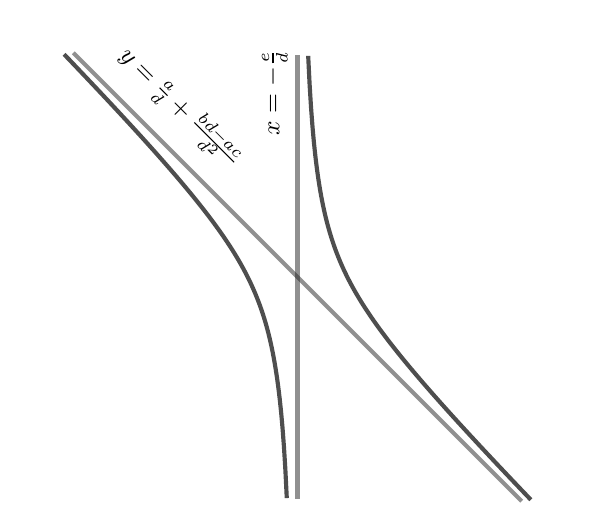
\begin{tikzpicture}
  \begin{axis}[
    font=\small\sf,
    axis lines = middle,
    axis line style={draw=none},
    % xlabel=$x$, ylabel=$y$,
    % xlabel style={below, font=\small\sf},
    % ylabel style={left, font=\small\sf},
    % ymin=-5.65, ymax=7.65,
    % ymin=-5.65, ymax=7.65,
    % width=12cm, height=8cm,
    xtick={},
    xticklabels={},
    xtick style={draw=none},
    ytick={1},    
    yticklabels={}, 
    ytick style={draw=none},  
    tick label style={font=\footnotesize\sf},
    clip=false,
    axis equal,
  ]

    % \node[originlabel] at (axis cs:0,0) [below right] {$O$};
    % \node at (axis cs:-5,0) [above] {$-5$};
    % \node at (axis cs:0,5/2) [left] {$\frac{5}{2}$};    
    % \node at (axis cs:2/3,0) [below] {$\frac{2}{3}$};
    % \node at (axis cs:2,0) [above] {$2$};
    % \node at (axis cs:0,-1) [left] {$-1$};
    % \node at (axis cs:0,-9/2) [left] {$-\frac{9}{2}$};
    % \node at (axis cs:0,-2) [left] {$-2$};
    % \node at (axis cs:4,0) [above] {$4$};
    % \node at (axis cs:9,0) [above] {$9$};
    % \node at (axis cs:2,-1) [below] {$I$};

    \addplot[domain=-5:5,
    restrict y to domain=-4.5:4.5, 
    samples=350, line width=1.5pt, color=den-2, opacity=.8] 
        {-x+1/x};
    \addplot[domain=-4.5:4.5,
    restrict y to domain=-5:5, 
    samples=350, line width=1.5pt, color=den-2, opacity=.5] 
        {-x};
    % \addplot[domain=-5:5,
    % restrict y to domain=-5:5, 
    % samples=350, line width=1.5pt, color=den-2, opacity=.8] 
    %     {-1/x};
    % \addplot[dashed, domain=-5:5,
    % restrict y to domain=-5:5, 
    % samples=350, line width=1.5pt, color=den-2, opacity=.5] 
    %     {x};
    % \addplot[dashed, domain=-5:5,
    % restrict y to domain=-5:5, 
    % samples=350, line width=1.5pt, color=den-2, opacity=.5] 
    %     {-x};
    \addplot[smooth, line width=1.5pt, color=den-2, opacity=.5] coordinates {
        (0,-4.45)
        (0,4.45)
        };
    \node[
    rotate=90, 
    above right,
    % font=\small\sffamily, % Kiểu font
    % color=den-2!80 % Màu chữ, có thể điều chỉnh độ đậm nhạt
    ] at (axis cs:0,2.65) {$x=-\frac{e}{d}$}; % Đặt tại tâm đường thẳng
    
    \node[
    rotate=-45,
    below,
    % font=\small\sffamily, % Kiểu font
    % color=den-2!80 % Màu chữ, có thể điều chỉnh độ đậm nhạt
    ] at (axis cs:-2,3.75) {$y=\frac{a}{d}+\frac{bd-ac}{d^2}$}; % Đặt tại tâm đường thẳng    
  \end{axis}
\end{tikzpicture}

\end{document}
